%!TEX root = thesis.tex
\chapter{Appendix}
\section{Evaluation of \acs{PID} Controller}
Although the scope of this thesis does not focuses on controller design and
tuning, a brief evaluation of the implemented \ac{PID} controller is given in
this section. By systematically exploring different values for the
\ac{PID} parameters, the final system applies $K_P = -0.09$, $K_I = 0$ and
$K_D = -28$. Figure \ref{fig:demo_pid} shows a tracking of the ball for two
applications.
\begin{figure}
	\centering
	\begin{subfigure}{0.49\textwidth}
		\centering
		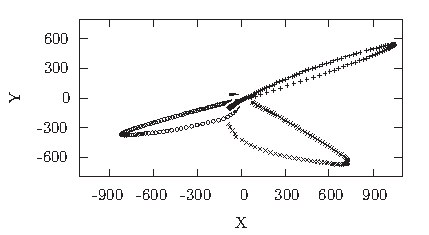
\includegraphics[width=\textwidth]{../figures/eval_pos}
		\caption{Balancing of ball in the center}
		\label{fig:eval_pos}
	\end{subfigure}
	\begin{subfigure}{0.49\textwidth}
		\centering
		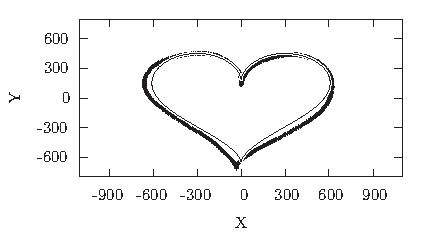
\includegraphics[width=\textwidth]{../figures/eval_traj}
		\caption{Following of a fixed trajectory}
		\label{fig:eval_traj}
	\end{subfigure}
	\caption{Captures of ball's movement controlled by \acs{PID} controller}
	\label{fig:demo_pid}
\end{figure}
For figure \ref{fig:eval_pos} the ball is balanced at the center of the plate
and any external disturbance is compensated, with the aim to keep the ball on
the plate. The figure shows a slight overshoot at the center and, due to a
missing integral term, never reaches the absolute center. Since the ball has a
relatively high initial friction, a large angle is needed to give the ball an
initial impulse. It then destabilizes and never reaches a resting position.
Therefore, a small inaccuracy for its final position is acceptable.
Additionally to the balancing of the ball in the center, figure
\ref{fig:eval_traj} shows an exemplary trajectory for the ball to follow.
Again, an inaccuracy from the desired trajectory in the direction of movement
is apparent. The trajectory is achieved by changing the target position of the
ball over time and adjusting the \ac{PID} controller to avoid the so-called
derivative kick.